% Faz com que o ínicio do capítulo sempre seja uma página ímpar
\cleardoublepage
% Inclui o cabeçalho definido no meta.tex
\pagestyle{fancy}

% Números das páginas em arábicos
\pagenumbering{arabic}

%espaco entre linhas
\onehalfspacing

\chapter{Conceitos Computacionais}\label{cap2}

\section{Escalonamento}\label{cap2:escalonamento}

Escalonamento é um processo de tomada de decisão que é usado como base em muitas indústrias manufatureiras e serviços industriais. Ele lida com a alocação de recursos para tarefas a fim de fornecer períodos de tempo a cada tarefa  e o fim é otimizar um ou mais objetivos~\citep{pinedo2012scheduling}.

Encontrar um escalonamento significa encontrar, para cada tarefa, uma alocação de um ou mais intervalos de tempo, em uma ou mais máquinas. O problema de escalonamento correspondente é encontrar um escalonamento que satisfaça um determinado conjunto de restrições.

Em um ambiente genérico de fabricação, o papel do escalonamento das tarefas é 
destacado nas ordens de serviço que são lançadas na configuração da fabricação,
em forma de tarefas com datas de entrega associadas. Essas tarefas 
frequentemente devem ser processadas em máquinas em uma dada ordem ou 
sequência. Os processamentos das tarefas podem atrasar, se certas máquinas 
estiverem ocupadas. Eventos imprevistos no chão-de-fábrica, tais como quebra de 
máquinas ou tempos de processamento maiores que os previstos, também devem 
ser levados em consideração, desde que esses eventos venham a impactar 
diretamente o escalonamento das tarefas. Neste ambiente, o desenvolvimento de um escalonador de tarefas detalhado ajuda a manter a eficiência e o controle das 
operações. 

O chão-de-fábrica não é a única parte da organização que impacta o 
processo de escalonamento. O escalonador também é afetado pelo processo de 
planejamento da produção que lida com o planejamento a médio e a longo prazos 
para toda a organização. Esse processo tenta otimizar toda linha de produtos da 
empresa e a alocação de recursos baseados em seus níveis de estoque, previsões 
de demanda e necessidades de recursos. As decisões tomadas neste nível mais alto 
de planejamento podem impactar o processo de escalonamento diretamente. 

Um exemplo de escalonamento é na indústria de semicondutores  no qual o objetivo é maximizar o tempo de utilização dos equipamentos e minimizar o tempo ocioso e de configuração dos mesmos~\citep{pinedo2012scheduling}.

Na computação o escalonamento está associado a utilização dos recursos da máquina como por exemplo a CPU. Existem vários algortimos de escalonamento entre eles~\citep{tanenbaum2006sistemas}:
\begin{itemize}
	\item FIFO \textit{(First In, First Out)}. A primeira tarefa a chegar será a primeira a ser executada.
	\item SJF \textit{(Shortest Job First)}. A tarefa mais curta tem ganhará o recurso, e uma fila em ordem de tamanhos da menor para a maior é feita atrás da menor.
	\item Round Robin. Todas as tarefas recebem um tempo de processamento, esse tempo é chamado de quantum.

\end{itemize}


\subsection{Notação dos problemas de escalonamento}

Nesta seção são apresentados uma breve introdução a notação associada aos problemas de escalonamento:

\begin{itemize}
\item Tempo de execução ($p_{ij}$) tempo necessário para a execução da tarefa $t_i$ na máquina $m_j$. Denotado apenas por $p_i$ se todas as máquinas forem idênticas
\item Data de disponibilidade ($r_i$) instante em que a tarefa $t_i$ se torna disponível para ser executada
\item Prazo ($d_i$) instante de tempo no qual a tarefa $t_i$ deve estar pronta
\item Peso ($w_i$) normalmente indica um fator de prioridade da tarefa $t_i$
\end{itemize}

A notação utilizada para representar os problemas de escalonamento, é representada pela tripla:   

$\alpha | \beta | \gamma$

$\alpha$ 	que descreve os recursos disponíveis

$\beta$ que descreve as tarefas a serem executadas

$\gamma$ que descreve o critério de otimização

$\alpha$ pode ser representado por:

\begin{itemize}
\item 1 uma única máquina
\item $P$ ou $P_m$ m máquinas paralelas idênticas cada tarefa $t_i$ pode ser processada em qualquer uma das $m$ máquinas por $p_i$ unidades de tempo, se uma tarefa só puder ser executada em um subconjunto das máquinas, a restrição será indicada no campo 
\item $P \infty$ ou $\overline{P}$ é o número ilimitado de máquinas idênticas
\end{itemize}

$\beta$ pode ser representado por:
\begin{itemize}
\item $Q_m$ máquinas paralelas uniformes no qual $m$ máquinas  operam com 
velocidades iguais (a máquina $m_j$ opera com velocidade $v_j$) $p_{ij} = p_i=v_j$
\item $R_m$ máquinas paralelas não-relacionadas, $m$ máquinas diferentes em paralelo
\item $p_{ij} = p_i=v_{ij}$, onde $v_{ij}$ é a velocidade da tarefa $t_i$ na máquina $m_j$
\end{itemize}


\subsection{Classes de Escalonamento}

Problemas de escalonamento podem ser divididos em classes, tais como escalonamento sem atrasos, escalonamento ativo e escalonamento semi-ativo. Essas classes agrupam os modelos de escalonamento e facilitam a forma de analisar o problema.

\subsubsection{Escalonamento sem atrasos}

 Um escalonamento válido é dito sem atraso, se nenhuma máquina fica inativa, ou seja, ociosa, quando existem tarefas disponíveis para serem executadas.

\subsubsection{Escalonamento ativo}

Os algorirmos de escalonamento podem ser preemptivos e não preemptivos. Preemptivo significa que o algoritmo permite que um processo seja interrompido durante a sua execução, para posteriormente ser retomado.

Um escalonamento é ativo se não for possível, apenas trocando a ordem das tarefas/operações em uma máquina, construir um outro escalonamento onde ao menos uma tarefa termine mais cedo e nenhuma outra tarefa seja atrasada.

\subsubsection{Escalonamento semi-ativo}

Um escalonamento é dito semi-ativo se nenhuma tarefa/operação pode terminar mais cedo sem que a ordem do processamento das tarefas de alguma máquina seja mudada.

\subsection{Classificação dos problemas de escalonamento}
Os problemas de programação de operações em máquinas vêm sendo caracterizados por diversos autores em diferentes formas, dentre eles: Baker, 1974; Blazewicz et al., 1996; Conway et al., 1967; French, 1982; Graves, 1981 e Pinedo, 2008.

Em situações de escalonar tarefas nas máquinas disponíveis surgem problemas complexos. Pois, as restrições tecnológicas e a medida de desempenho do escalonador devem ser especificadas. As restrições tecnológicas são determinadas principalmente pelo fluxo das tarefas nas máquinas.

Neste contexto, Maccarthy e Liu (1993) classificam os problemas de programação de operações da seguinte forma:
 
\begin{itemize}
\item \textbf{Máquina única} - existe somente uma única máquina disponível para a execução das tarefas;
\item \textbf{Flow shop} - em que todas as tarefas possuem o mesmo fluxo de processamento em todas as máquinas;
 \item \textbf{Job shop} - em que todas as tarefas possuem um roteiro específico de processamento, determinado para cada tarefa;
 \item \textbf{Open shop} - em que não existem roteiros de processamento preestabelecidos para as tarefas;
 \end{itemize}

%Cap 3

O problema do sequenciamento em uma única máquina quase sempre parte de um problema de programação complexo.  Segundo Pinedo (2008), os problemas do sequenciamento em uma única máquina  muitas vezes têm propriedades que os de em máquinas em paralelo ou em série  não possuem. Os resultados que podem ser obtidos para os problemas do  sequenciamento em uma única máquina não só fornecem o conhecimento para o ambiente de uma única máquina, como também fornecem base para heurísticas  aplicáveis a ambientes mais complexos. 

Na prática, os problemas de escalonamento em ambientes mais complicados são frequentemente decompostos em subproblemas de uma única máquina. 

Por exemplo, um ambiente complexo, com um único gargalo, pode dar origem a um modelo de sequenciamento em uma única máquina. Dessa forma, o problema do sequenciamento em uma única máquina é importante por diversas razões, dentre elas pode-se citar: 

\begin{itemize}
\item O processo de aprendizado, já que o problema de escalonamento em uma única máquina  pode ilustrar uma variedade de tópicos de escalonamento tornando modelos tratáveis. Esse problema fornece um contexto para que se  investigue muitas medidas de desempenho e técnicas de solução. Além disso, é uma base para o entendimento de  conceitos de escalonamento úteis para modelar sistemas mais complexos. 

\item Para entender completamente o comportamento de um sistema  complexo, é vital entender como funciona cada um de seus componentes e muito frequentemente o problema de uma única máquina aparece como componente elementar em um problema de escalonamento maior. 

\item Algumas vezes é possível resolver o problema de escalonamento em uma única máquina independentemente e então incorporar o resultado em um problema maior. Por exemplo, em um processo com múltiplas operações, frequentemente existe uma operação gargalo e o tratamento dessa operação gargalo, vista como uma análise de um problema de uma única máquina, determina as propriedades de todo o escalonamento. 

\end{itemize}

\subsection{Modelo de escalonamento para uma única máquina}

Ao lidar com os atributos para o modelo de uma única máquina, é  útil distinguir entre informações conhecidas previamente e informações que são geradas como resultados de decisões de escalonamento. A informação que é conhecida previamente serve como parâmetro de entrada para função de escalonamento e é usualmente conveniente usar letras minúsculas para denotar esse tipo de informação, são elas $\alpha | \beta | \gamma$.

Os prazos podem não ser pertinentes em certos problemas, mas estabelecer os prazos (deadlines) é um problema comum na indústria e o problema básico pode auxiliar na determinação do prazo de entrega. É conveniente usar letras maiúsculas para denotar as informações resultantes do escalonamento. 

\begin{itemize}

\item Tempo de Conclusão ($C_j$). O tempo no qual o processamento do trabalho $j$ é terminado. 

Os critérios quantitativos para escolher uma sequência são geralmente funções dos tempos de conclusão. Duas funções importantes são: 

\item Tempo de Fluxo (Flowtime) – $F_j$ – Tempo total que o trabalho $j$ fica no sistema: 

$F_j = C_j – r_j$
 
\item Defasagem (Lateness) – $L_j$ – Diferença entre a data de conclusão e o prazo do trabalho $j$, podendo assumir valores positivos ou negativos

É importante notar que a defasagem terá valor negativo quando uma tarefa é finalizada antecipadamente. Defasagens negativas podem representar serviços melhores do que solicitados, enquanto atrasos positivos representam, quase sempre, serviços piores do que requisitados. Em muitas situações, penalidades distintas e outros custos serão associados para defasagens positivas e para defasagens negativas. Dessa forma, tem-se as definições de Atraso (Tardiness) e Antecipação (Earliness): 

\item Atraso (Tardiness) – $T_j$ – é o quanto o trabalho $j$ atrasou em relação ao seu prazo, caso contrário será considerado zero:
 
$T_j = max\{0, L_j\}$ 

\item Antecipação (Earliness) – $E_j$ – é o quanto o trabalho $j$ é antecipado em relação ao prazo, caso contrário será considerado zero: 
 
$ E_j = max\{d_j – C_j, 0\} $
 
\item Makespan – $C_{max}$ – é definido como o maior dentre as datas de 
conclusão ($C_1, . . ., C_n$), ou seja, ao tempo de conclusão do último trabalho a sair do sistema ($C[n]$). Minimizar o makespan usualmente implica em uma boa utilização dos recursos. 

\end{itemize}


\section{Balancemento de Carga}\label{intro:carga}

O problema de balanceamento de carga é estudado por pesquisadores da área de Teoria de Escalonamento há mais de 50 anos. Em 1966, \citep{graham66} estudou o que chamou de "anomalias'' na execução de tarefas em processadores de velocidades diferentes. Ele mostrou, por exemplo, que a adição de novos processadores ou a troca de alguns processadores por outros de maior velocidade podem propiciar o desbalanceamento de carga e, portanto, não necessariamente implicam em um ganho no desempenho. Logo ficou clara a necessidade de algoritmos mais sofisticados para lidar com esse problema.  

O balanceamento de carga é uma técnica aplicada para distribuir a carga de trabalho entre dois ou mais servidores, enlaces de rede, CPU, ou outros recursos; a fim de otimizar a utilização destes recursos, maximizar o desempenho e evitar sobrecarga. Em geral o balanceamento de carga consiste em três fases~\citep{carga}. A primeira, consiste na coleta de informações. A segunda, busca determinar qual seria a distribuição ótima para o estado em que o sistema se encontra. E por fim a terceira fase, que a ação de balanceamento é executada. O balanceador de carga pode ter uma das seguintes classificações:

\begin{itemize}
\item Estático A regra de balanceamento é definida uma única vez, baseada em informações estáticas do sistema ou aplicações.

\item Dinâmico A regra de balanceamento é modificada em resposta ao estado atual do sistema ou das aplicações. O estado do sistema será constantemente atualizado e as decisões tomadas são baseadas nas informações atuais e possivelmente, dos estados anteriores do sistema.
\end{itemize}

Ao balancear a carga, tenta-se evitar que no sistema, existam simultaneamente máquinas com recursos subutilizados e máquinas com recursos super utilizados. Na maioria dos casos, realizar balanceamento de carga ótimo é impraticável, devido a complexidade computacional para resolver o problema. O problema de balanceamento de carga  é similar a problemas de alta complexidade computacional~\citep{virtual}, NP-Completo que não podem ser resolvido de maneira exata em tempo polinomial. Para contornar esta limitação, heurísticas ou algoritmos de aproximação, são usados para apresentarem soluções aproximadas do balanceamento de carga ótimo.


Distribuição de carga estática, também conhecida como planejamento determinístico, atribui um determinado trabalho a processador fixado. Toda vez que o sistema for reiniciado, a mesma tarefa no processador de ligação (atribuição de uma tarefa ao mesmo processador) é usada sem considerar as mudanças que podem ocorrer durante a vida útil do sistema. Além disso, a distribuição de carga estática pode também caracterizar a estratégia utilizada durante a execução, no sentido de que ele pode não resultar na mesma atribuição de tarefas no processador, mas atribui os postos de trabalho recém-chegados de uma forma sequencial ou fixa. Por exemplo, utilizando uma estratégia estática simples, os trabalhos podem ser atribuídos aos nós de uma maneira round-robin de modo que cada processador execute aproximadamente o mesmo número de tarefas. 

Balanceamento de carga dinâmico leva em conta que os parâmetros do sistema não podem ser conhecidos com antecedência e, por conseguinte, utilizando um esquema fixo ou estático irão eventualmente produzir resultados ruins. A estratégia dinâmica geralmente é executado várias vezes e poderá realocar um trabalho previamente escalonado para um novo nó com base na dinâmica atual do ambiente de sistema.

Os problemas tratados neste trabalho se restringem aos problemas que não apresentam dependência de dados entre si. A técnica ultilizada é chamada de decomposição de domínio. Que consiste em dividir um conjunto inicial em subconjuntos. O problema restringe a determinar a quantidade de dados que devem ser enviados a cada processador de forma a minimizar o tempo total de processamento em um ambiente de processadores heterogêneos. 

\subsubsection{Balanceamento de carga Distribuido e Centralizado}

Essa divisão geralmente cai sob o esquema de balanceamento de carga dinâmico, onde uma questão natural surge sobre o local onde a decisão é tomada. Políticas centralizadas armazenam informações globais em um local central e usa essas informações para fazer o escaonamento de decisões tomadas pelos que utilizam os recursos de armazenamento de um ou mais processadores. Este esquema é o mais adequado para sistemas em que as informações de estado de um processador individual podem ser facilmente coletados por uma estação central a baixo custo, e novos postos de trabalho que chegam a este local centralizado serão depois encaminhados para nós subseqüentes. A principal desvantagem deste sistema é que ele tem um ponto único de falha. 

Na programação distribuída, as informações de estado é distribuída entre os nós que são responsáveis na gestão dos seus próprios recursos ou distribuiem as tarefas que residem em suas filas a outros processadores. Em alguns casos, o sistema permite que os processadores ociosos atribuam tarefas a si mesmos em tempo de execução, acessando uma fila global compartilhada. Note-se que as falhas ocorrem em um determinado nó irão permanecer localizado e não pode prejudicar o funcionamento global do sistema. 

Em um escalonamento de balanceamento de carga local, cada processador pesquisa outros processadores em sua vizinhança e usa esta informação local para decidir sobre a transferência de carga. Esta vizinhança é geralmente indicada como o espaço de migração. O principal objetivo é minimizar a comunicação remota, bem como de forma eficiente equilibrar a carga sobre os processadores. No entanto, em um esquema de balanceamento global, informação global ou  parte da informação do sistema é utilizado para iniciar o balanceamento de carga. Este sistema exige uma quantidade considerável de informações a serem trocadas no sistema o que pode afetar sua capacidade de expansão.

No âmbito da escalonamento distribuído global dinâmico, dois mecanismos podem ser distinguidos, envolvendo o nível de cooperação entre as diferentes partes do sistema. No esquema não cooperativo ou autônomos, cada nó tem autonomia sobre o seu próprio escalonamento de recursos. Isto é, as decisões são tomadas independentemente do resto do sistema e, portanto, o nó pode migrar ou afetar funções baseadas no desempenho local. Por outro lado, na programação cooperativa, os processos trabalham em conjunto para um balanço global de todo o sistema. Decisões de escalonamento são feitas após considerar seus efeitos sobre algumas medidas efetivas globais (por exemplo, o tempo global de conclusão).

Esquemas adaptativos e não-adaptativos são parte das políticas de balanceamento de carga dinâmico. Em um esquema adaptativo, as decisões escalonadas levam em consideração o passado e o desempenho atual do sistema e são afetados pelas decisões anteriores ou alterações no ambiente. Se um (ou mais parâmetros) não se correlacionam com o desempenho do programa, que é ponderado menos próxima vez. No regime não-adaptativo, os parâmetros utilizados no escalonamento continuam os mesmos, independente do comportamento passado. 
	
Confusões podem surgir entre a distinção entre escalonamento dinâmico e escalonamento adaptativo. Uma solução dinâmica leva em conta informações ambientais na sua decisão, uma solução adaptativa (que também é dinâmica) leva em conta estímulos ambientais em consideração para modificar a própria política de escalonamento.



\section{GPUs}\label{intro:historico}

As GPUs vêm se mostrando uma excelente alternativa na área de computação de alto-desempenho para aplicações que exigem um alto grau de paralelismo~\citep{gpu}. GPUs modernas possuem dezenas de núcleos, cada um deles bastante simples, mas que utilizados em paralelo geram um alto poder computacional~\citep{cuda}.

Muitas aplicações já utilizam o poder de processamento das GPUs, exemplos são mecânica dos fluidos~\citep{fluido}, visualização científica~\citep{visualizacao},  aprendizado de máquina~\citep{Aprendizado}, entre outras. Devido ao relativo baixo custo de placas gráficas contendo GPUs, sua utilização é uma ótima alternativa para pesquisadores pertencentes a instituições com poucos recursos financeiros e com grande necessidade de recursos computacionais.


\section{CUDA}\label{intro:contexto}

\textit{Compute Unified Device Architecture} (CUDA)~\citep{cuda} é uma arquitetura de computação paralela desenvolvida pela Nvidia para processamento gráfico.
Com esta tecnologia é possível desenvolver não só aplicações convencionais de processamento gráfico, mas é possivel fazer programas de propósito geral, esta abordagem de se desenvolver programas de propósito geral em GPU é denominado GPGPU (\textit{General-Purpose Computing on Graphics Processor Units})~\citep{GPGPU}.

Através de linguagens de programação amplamente utilizadas na indústria é possível desenvolver variadas aplicações que se beneficiam do alto poder de processamento das placas gráficas. A principal linguagem utilizada para o desenvolvimento em CUDA é a linguagem de
programação C, que mundialmente é a mais amplamente utilizada. O principal mérito do CUDA é a facilidade que se tem para acessar todos recursos da placa gráfica.

%%%%%%%%%%%%%%%%%%%%Revisar
CUDA foi lançado pela NVIDIA em novembro de 2006~\citep{cuda}. Sua proposta foi criar uma arquitetura de computação paralela de propósito geral. A justificativa para isso foi aproveitar a plataforma de computação paralela das placas gráficas para resolver diversos algoritmos
computacionais eficientemente. O aplicativo produzido sobre a API CUDA pode ser um algoritmo em linguagem C, OpenCL, Fortran, C++ e DX11, não havendo limitações para o suporte de novas linguagens. 

\begin{figure}[htb]
	\begin{center}
	\centering
			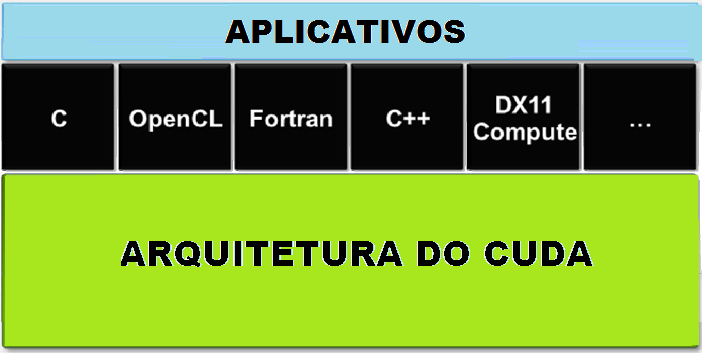
\includegraphics[scale=0.6]{LingSuportadas.png}
	\label{fig: lingSuportadas}
	\caption{Linguagens Suportadas(adaptado de~\citep{cuda})}
	\end{center}
\end{figure}

A arquitetura NVIDIA CUDA se baseia tanto em componentes de hardware como de software~\citep{cuda}. A parte que entendemos por software é a executada na CPU, formada por um algoritmo seqüencial escrito comumente na linguagem C ou alguma outra que é suportada por CUDA. A parte do hardware é formada pelo código compilado por CUDA para torná-lo um kernel. \textit{Kernel} são blocos que especificam parte do algoritmo em que se deseja a
paralelização. Ele também pode ser tratado como um código que pode ser utilizado pela GPU para chamar outros kernels nela ou em outra GPU.

A GPU contém milhares de threads. CUDA faz a formatação do código de uma maneira que threads sejam alocadas paralelamente e o usuário usufrua dessa característica, podendo fazer chamadas de kernel que serão independentes entre si, o que permite a GPU rodar vários algoritmos.

Podemos ver na Figura 1.2 a diferença de potencial que uma GPU, com seu paralelismo, possui em relação a um processador (CPU):

\begin{figure}[!htb]
	\begin{center}
	\centering
			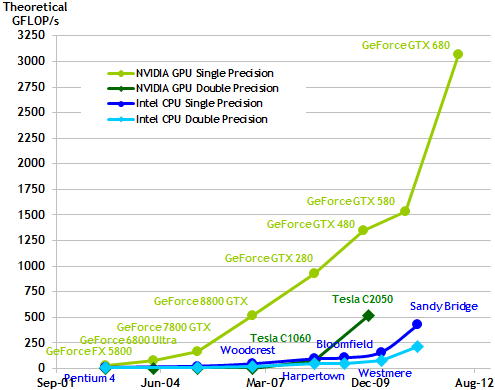
\includegraphics[scale=0.8]{ImageSub.png}
	\label{fig: graficosCuda1}
	\caption{Operações de Ponto Flutuante por segundo para CPU e GPU(adaptado de~\citep{cuda})}
	\end{center}
\end{figure}

Na figura \ref{fig: graficosCuda1} gráfico temos informações sobre o pico de operações por ponto flutuante. A GPU alcança a casa de TFlops/s, e a CPU apresenta um desempenho baixo mesmo comparado a arquiteturas de GPUs anteriores que não são compatíveis com CUDA.

\begin{figure}[!htb]
	\begin{center}
	\centering
			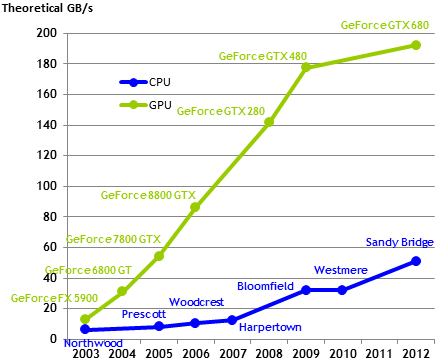
\includegraphics[scale=0.8]{ImageSub2.png}
	\label{fig: graficosCuda2}
	\caption{Tamanho de banda de memória para CPU e GPU(adaptado de~\citep{cuda})}
	\end{center}
\end{figure}

A GPU é voltada para computação intensiva, com alta paralelização, que são características do problema de renderização gráfica. Além disso, sua arquitetura é especializada no processamento deste tipo de dados e não no controle de fluxo. Podemos visualizar essa diferença quando
observamos a Figura 1.3.

\begin{figure}[!htb]
	\begin{center}
	\centering
			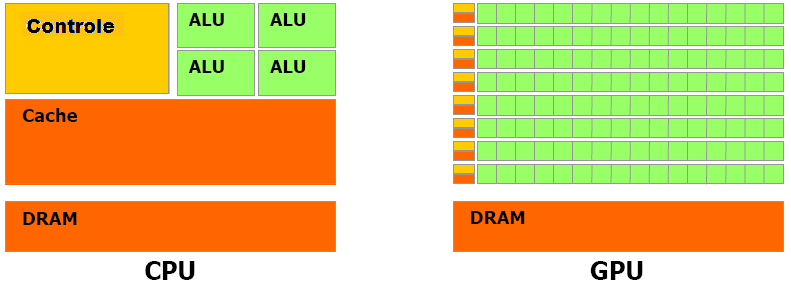
\includegraphics[scale=0.6]{transistores.png}
	\label{fig: transistores}
	\caption{Quantidade de transistores para processamento de dados(adaptado de~\citep{cuda})}
	\end{center}
\end{figure}

A quantidade de transistores utilizados para fazer processamento (ALU - \textit{Arithmetic Logic Unit}) é bem maior na GPU que na CPU. A arquitetura da CPU ainda está dividida em enormes blocos que contêm um componente de controle de fluxo e um de memória cache. No caso da GPU, o mesmo programa é executado em muitos elementos em paralelo. Dessa maneira, não possui um sofisticado componente de controle de fluxo, porém, oferece uma grande intensidade de computação aritmética. Além disso, a cache se torna pequena na GPU diminuindo a latência para execução de cada grande bloco de ALU's, diferente da CPU que contém uma cache enorme, obtendo uma latência alta para acesso. Possuindo uma unidade de controle, um componente de cache e um conjunto enorme de ALU's, é possível obter a estrutura de vários grupos de
cores. Podemos assim certificar que a GPU é um manycore, apresentando de 32 até 128 cores dependendo do modelo. Essa subdivisão de cores na GPU é chamada de \textit{Stream Processing}.

Um ponto importante a ser lembrado é que, para a execução na GPU, o algoritmo paralelizado não pode ter muita dependência de dados em cada passo de computação, pois a GPU não faz paralelização de tarefas e sim de processamento de dados. Caso essa otimização não seja feita no algoritmo, a GPU tem seu desempenho bastante afetado.

Com relação à hierarquia de compilação para o CUDA, a Figura 1.4 ilustra a arquitetura da sua pilha de software.

\begin{figure}[!htb]
	\begin{center}
	\centering
			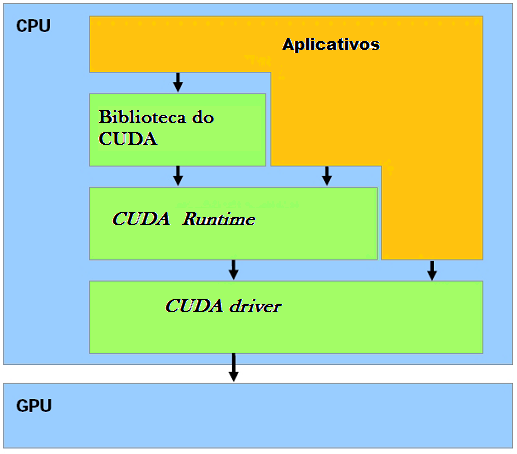
\includegraphics[scale=0.6]{pilhaSoftware.png}
	\label{fig: pilhaSoftware}
	\caption{Pilha de Software(adaptado de~\citep{cuda})}
	\end{center}
\end{figure}

Essa pilha de software mostra a hierarquia de execução de CUDA. A API de CUDA fornece suporte a diversas funções matemáticas, bibliotecas, suporte ao runtime e ao driver.

O CUDA \textit{runtime} ~\citep{cuda} é a camada de alto nível de programação, enquanto a camada do driver é a camada baixa para manipulação de dados. O CUDA driver gerencia e otimiza os recursos relacionados diretamente à GPU. CUDA é baseada em programação paralela, permitindo milhares de threads executando uma mesma tarefa. Neste caso, a GPU funciona como um co-processador da CPU, a qual chamamos de \textit{HOST} e a GPU de \textit{DEVICE}.

CUDA usa como base a linguagem C~\citep{cuda}, que permite uma curva rápida de aprendizado. Nela deve-se criar funções desejadas que CUDA otimiza e paraleliza na GPU. Essas funções são chamadas de kernel. A seguir, observamos um exemplo de um código simples, em seguida, uma explanação sobre cada aspecto inerente ao entendimento seqüencial desse código.


\begin{verbatim}
__global__ void matAdd(float A[N][N], float B[N][N],
float C[N][N])
{
    int i = threadIdx.x;
    int j = threadIdx.y;
    C[i][j] = A[i][j] + B[i][j];
}


int main()
{
    // Kernel invocation
    dim3 dimBlock(N, N);
    matAdd<<<1, dimBlock>>>(A, B, C);
}

\end{verbatim}

Nesse código temos uma função matAdd que apresenta uma tag \textit{\_\_global\_\_} antes da definição da função. Essa tag define ao compilador que esse bloco será paralelizado na GPU.  Esta função recebe três matrizes de tamanho N por N, onde cada thread nos eixos x e y serão responsáveis por somarem as matrizes A e B, sendo atribuido o resultado da soma na matriz C.  Caso fosse desenvolvido um código similar no modo convencional, teria que aninhar dois laços de forma a percorrer todos os indices das matrizes. É claro, a diferença na forma de implementar e tratar o problema.

A função \textit{main} faz a invocação do método. Ele se localiza no HOST e o código é executado na GPU (DEVICE). Em um computador podemos encontrar mais que uma GPU, neste caso elas serão chamadas de DEVICE 0, DEVICE 1, etc. O kernel é acionado colocando uma \textit{tag} de configuração antes da declaração dos parâmetros, "$<<< >>>$". Há três parâmetros possíveis na configuração: a configuração do tamanho das \textit{grids} (A), a configuração do tamanho dos blocos (B) e a quantidade de memória compartilhada que se deseja utilizar no algoritmo (Ns). Isso gera uma configuração genérica "$<<<A,B,Ns >>>$".

No main, antes da invocação, declaramos um tipo de variável definida pelo CUDA chamada "dim3". A variável criada dimBlock terá três dimensões e cada uma dessas dimensões representará a dimensão de um bloco. No exemplo, teremos um bloco com tamanho $N$ para dimensão $x$, tamanho $N$ para dimensão $y$ e a dimensão $z$ que foi omitida tem tamanho 1. Desta forma, seguindo a lógica de desenvolvimento da aplicação é possível construir algoritmos paralelizados na GPU.


A arquitetura CUDA é baseada em \textit{arrays} escaláveis de multithreads SMs, ou thread Batching. Ele é um \textit{batch} de threads que o kernel executa e organiza em grids de threads block. Uma thread block é um batch de threads que cooperam entre si para compartilhar eficientemente as informações que serão processadas. Essa eficiência vai desde o compartilhamento (cópia da DRAM GPU para a memória compartilhada e vice-versa) dessa informação através da memória compartilhada, até a sincronização de execução para o acesso a essa memória.

Cada thread é identificada através de ID única, chamada thread ID. Há um número limitado de threads por bloco. Porém, um bloco de mesma dimensão e tamanho pode ser executado por um mesmo kernel fazendo um grid de blocos, aumentando ainda mais a quantidade de threads sendo executados em paralelo. Vale salientar que as threads de blocos diferentes não podem se comunicar.
Cada bloco é identificado por um block ID, e tem sua ID única em relação ao grid.

\begin{figure}[!htb]
	\begin{center}
	\centering
			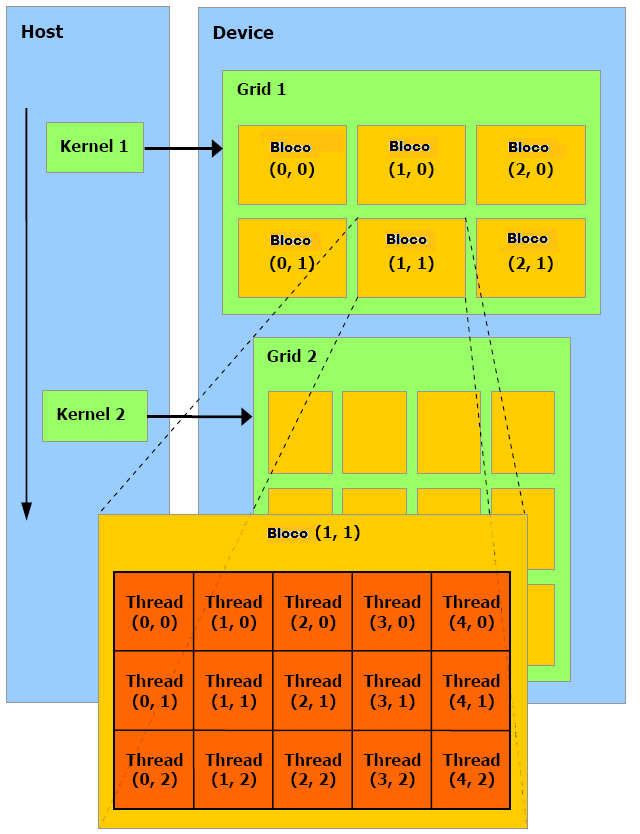
\includegraphics[scale=0.6]{ThreadBatching.png}
	\label{fig: ThreadBatching}
	\caption{Batching de Threads(adaptado de~\citep{cuda})}
	\end{center}
\end{figure}

Um multiprocessador é um nome formalizado para threads. Ele consiste de oito cores de processadores escalares, duas unidades de funções especiais transcendentais, uma unidade de controle de instruções multithread e uma memória compartilhada on-chip.

O multiprocessador cria, gerencia, e executa threads concorrentes com custo nulo de hardware no âmbito de gerenciamento de processos. Para gerenciar centenas de threads rodando em diferentes programas, o multiprocessador nas últimas versões de CUDA emprega o SIMT. O multiprocessador mapeia cada thread a um core de processador escalar, que executa independentemente suas próprias instruções e tem seu próprio estado de registradores.

Esse multiprocessador SIMT cria, gerencia, escalona e executa grupos de 32 threads paralelas chamadas de warps. Threads individuais que compõem o SIMT \textit{warp} podem começar sua execução juntas no mesmo programa, mas estão livres para ramificarem e executarem de forma autônoma. Contudo, se alguma thread ultrapassar a dependência condicional da ramificação, ela será desabilitada. 

A arquitetura SIMD(\textit{Single Instruction Multiple Data}) é implementada como um conjunto de múltiplos processadores que tem a capacidade de, com uma única instrução, em um mesmo ciclo de clock, processar várias informações.

\begin{figure}[!htb]
	\begin{center}
	\centering
			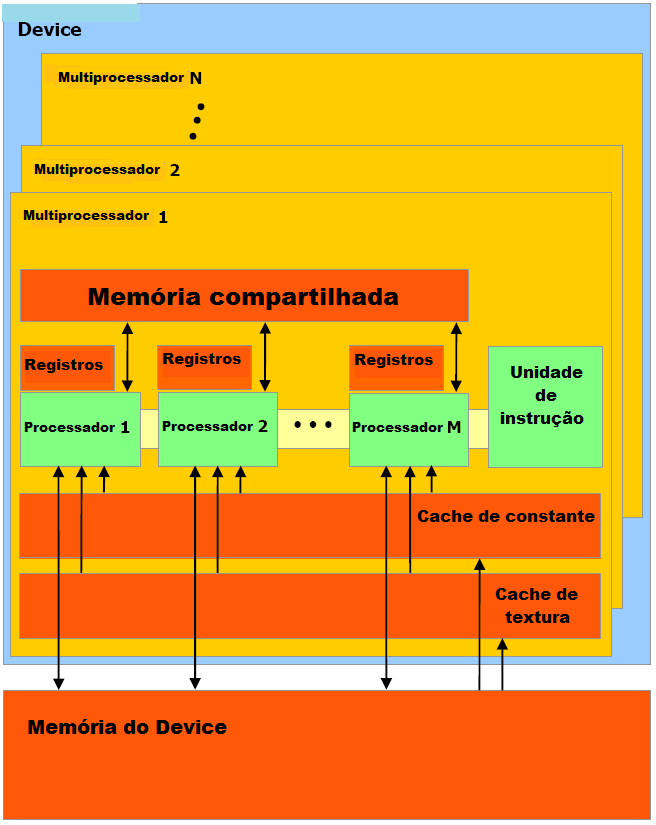
\includegraphics[scale=0.6]{SIMT.png}
	\label{fig: SIMT}
	\caption{Conjunto de Multiprocessadores e Organização das Memórias(adaptado de~\citep{cuda})}
	\end{center}
\end{figure}

Como podemos observar cada multiprocessador possui: um conjunto de registradores de 32-bit, cache paralelo ou memória compartilhada que é partilhada com os outros processos, uma cache constante e outra de textura apenas para leitura. A memória local e global não é "cacheada" e pode ser escrita e lida pelos processos.
Um ponto forte de CUDA é que há uma separação na memória DRAM entre o HOST e o DEVICE. A API de CUDA fornece uma forma de transmissão de alta performance para transferir os dados entre esses dispositivos usando \textit{High Performance} (DMA), ou DMA de alto desempenho.

\begin{figure}[!htb]
	\begin{center}
	\centering
			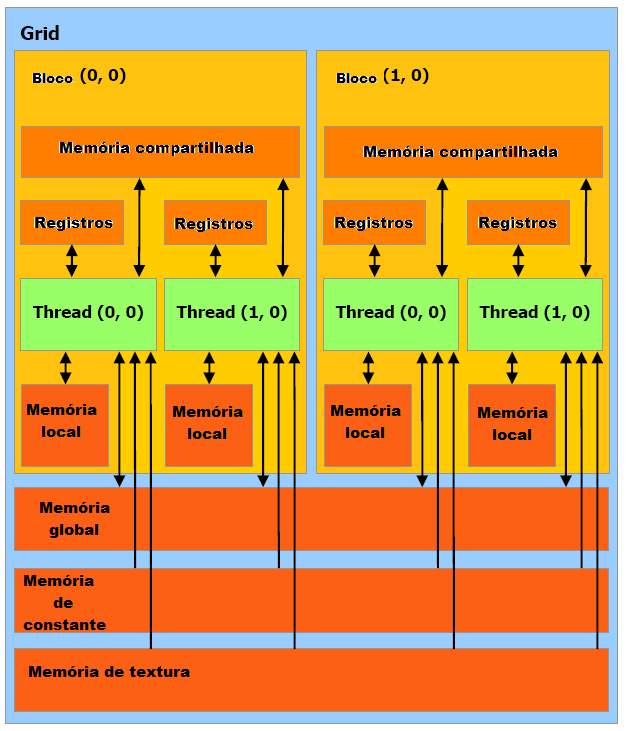
\includegraphics[scale=0.6]{HierarquiaMemoriasCuda.png}
	\label{fig: HierarquiaMemoriasCuda}
	\caption{Hierarquia de memórias da GPU(adaptado de~\citep{cuda})}
	\end{center}
\end{figure}


\section{Suporte ao Paralelismo de Tarefas}
Diversas ferramentas de programação suportam paralelismo de tarefas em CPUs multicore. Recentemente, alguns trabalhos em andamento têm buscado oferecer suporte a esse paradigma também em sistemas híbridos compostos por CPUs e GPUs.




\subsection{StarPU}

 StarPU~\citep{starpu} é um \textit{framework} para o escalonamento de tarefas em
plataformas heterogêneas, onde informações sobre o modelo de desempenho das
tarefas podem ser passadas para orientar as políticas de escalonamento. Os dois
princípios básicos da StarPU são (i) as tarefas podem ter várias implementações,
para alguns ou para cada uma das várias unidades de processamento heterogêneas
disponíveis na máquina, e (ii) a transferência de dados para estas unidades de
processamento são tratadas de forma transparente pelo StarPU. Escalona dinamicamente
tarefas em todos as unidades de processamento. Evita as transferências de dados  desnecessário entre aceleradores. Aceita tarefas que podem ter várias implementações. Fornece uma camada alto nível de gerenciamento de dados. Quando uma tarefa é submetida, pela primeira vez entra em um "pool" de "Tarefas congeladas" até que todas as dependências sejam atendidas. Em seguida, a tarefa é "empurrado" para o escalonador. Algumas politicas de escalonamento foram testadas utilizando a interface Starpu, entre elas greedy, no-prio, ws, w-rand, heft-tm. 

A estratégia greedy, no-prior e ws são estratégias gulosas, no qual  a greedy se diferencia da no-pior pois a greedy tem suporte a prioridades, então pode ponderar pesos de prioridade a tarefas enquanto na no-prior não é possível. E a ws é uma estratégia gulosa baseada no "work-stealing" que é uma estratégia que consiste em as unidades de processamento terem uma pilha de tarefas e se houver o término das tarefas pode haver o "roubo" da tarefa de outras unidades. 

Na estratégia w-rand, cada unidade de processamento está associada com uma relação que pode ser considerada como um fator de aceleração. Cada vez que uma tarefa é submetida, uma das unidades de processamento é selecionada com probabilidade proporcional à sua relação. Essa relação pode, por exemplo, ser definida pelo programador, ou ser medida com benchmarks de referência. A estratégia w-rand é normalmente adequado para tarefas independentes de igual tamanho.

A tarefa de distribuir uniformemente sobre as unidades de processamento baseado na velocidade não significa necessariamente fazer sentido para as tarefas que não são igualmente custosas, ou quando existem dependências entre eles. Assim, os programadores podem especificar um modelo de custo para cada tarefa. Este modelo pode por exemplo representar a quantidade de trabalho e ser usado em conjunto com a velocidade relativa de cada um das unidades de processamento. É também possível modelar diretamente o tempo de execução de cada uma das arquiteturas. Usando esses modelos, implementa-se a estratégia heft-tm. Dada a sua duração esperada nas várias arquiteturas, é atribuída uma tarefa para as unidades de processamento que minimiza o tempo de término, no que diz respeito à quantidade de trabalho já atribuída a esta unidade de processamento.

 O StarPU propõe uma abordagem de tarefas independente da arquitetura base. São definidos codelets como uma abstração de uma tarefa que pode ser executada em um núcleo de uma CPU multicore ou submetido a um acelerador. Cada codelet pode ter múltiplas implementações, uma para cada arquitetura em que o codelet pode ser executado, utilizando as linguagens ou bibliotecas específicas para a arquitetura alvo. Uma aplicação StarPU é descrita como um conjunto de codelets com suas dependências de dados.

StarPU é um sistema de execução unificado que consiste em um software e uma API de tempo de execução que tem como objetivo permitir que os programadores de aplicações com alto custo  computacional explorem mais facilmente o poder de dispositivos disponíveis, com suporte a CPUs e GPUs. Submissões de tarefas são manipuladas pelo escalonador do StarPU, e a consistência dos dados é garantida através de uma biblioteca de gerenciamento de dados. 
No entanto, uma das principais vantagens perante a outras bibliotecas é que o StarPU tenta reduzir o custo da transferência de dados. Isso é feito usando as informações do histórico de cada tarefa e, de acordo com as decisões do escalonador, que de forma assíncrona prepara as dependências de dados, enquanto o sistema está ocupado realizando a computação de outras tarefas. 

A API do StarPU apresenta uma certa terminologia bem definida, descrita a seguir:

\begin{itemize}
	\item Manipulador de Dados (Data Handle): Referência a blocos de memória. A alocação do espaço requerido, e a entrega de informações sobre a transferência de dados para cada dispositivo.
	\item Codelet: Descreve uma função computacional que pode ser implementada em um ou mais arqquiteturas, tais como CPUs, CUDA ou OpenCL. Também armazena informação sobre a quantidade e tipos de dados em buffers que podem ser recebidos.
	\item Tarefa (Task): É definido como a  associação entre um codelet e um conjutno de data handles.
	\item Partição (Partition): A subdivisão de um data handle em pequenos pedaços, de acordo com a função de divisão, que pode ser definida pelo usuário.
	\item Trabalhador (Worker): Um elemento processador, tal como um core CPU, gerenciado pelo StarPU para excutar Tasks;
	\item Escalonador (Scheduler): A biblioteca responsável pela atribuição das tarefas aos trabalhadores, com base em uma política de escalonamento bem definida.

\end{itemize}


\subsubsection{Escalonador de tarefas}

O \textit{framework} StarPU emprega um modelo de programação baseado em tarefas. Kernels computacionais devem ser encapsuladas dentro de uma tarefa. StarPU vai lidar com a decisão de onde e quando a tarefa deve ser executada, com base em uma política de escalonamento de tarefas, e as implementações disponíveis para cada tarefa. Uma tarefa pode ser implementada de várias formas, tais como a CPU ou CUDA. Várias implementações para o mesmo tipo de dispositivo podem também ser utilizadas. Isso permite que StarPU automaticamente selecione a implementação apropriada, mesmo entre diferentes arquiteturas de CPU. Ao enviar uma tarefa, StarPU vai usar o escalonador escolhido para selecionar qual das implementações disponíveis serão utilizadas. A decisão varia de escalonador para escalonador, mas pode levar em conta informações como a atual disponibilidade de cada recurso, o modelo de desempenho já obtido para essa tarefa, e as estimativas sobre as transferências de dados necessários para resolver as dependências. A vantagem do uso de StarPU perante as outras ferramentas é a capcacidade e facildade de alteração do escalonador. A API do StarPU apresenta uma grande variedade de funções que permitem agilizar a implementação de um novo escalonador.

Os dados manipulados por uma tarefa são transferidos automaticamente quando necessário entre os vários dispositivos, assegurando a consistência de memória e liberando o programador de lidar com questões de escalonamento, transferência de dados e outros requisitos associados.

\subsubsection{Dependências}

StarPU cria automaticamente um grafo de dependência de todas as tarefas apresentadas, e os mantém em um conjunto de "tarefas congeladas", passando-as para o escalonador uma vez preenchidas todas as dependências. 

Dependências podem ser implicitamente dadas pelos dados manipulados pela tarefa. Cada tarefa recebe um conjunto de buffers, cada uma correspondendo a uma parte dos dados geridos pela  biblioteca de gerenciamento de dados do StarPU, e irá esperar até que todos os buffers estiverem prontos para ler.

Isso inclui as possíveis transferências de dados que são necessárias para atender as dependências, neste caso diferentes tarefas que dependem dos mesmos dados estão programados para rodar em diferentes nós computacionais. StarPU se certificará automaticamente das transferências de dados necessárias entre cada execução da tarefa para garantir a consistência dos dados. 

Além de dependências de dados implícitos, outras dependências pode ser dados explicitamente a fim de forçar explicitamente a ordem de execução de um determinado conjunto de tarefas.


\subsubsection{Modo de acesso aos dados}

Cada dependência de dados que é explicitamente definida em uma tarefa, pode ter um modo de acesso diferente. Os dados podem ser usados em somente leitura, somente escrita ou no modo leitura e escrita. Este modelo descreve um tipo de padrão de mútua exclusão, onde um bloco de dados pode ser acessado simultaneamente por qualquer número de leitores, mas deve ser acessado exclusivamente por um escritor. 

StarPU usa esse conceito para otimizar ainda mais os cálculos de dependência de dados. Se várias tarefas escalonadas dependem dos mesmos dados, então apenas com o acesso a leitura de dados, a dependência não deve bloquear as múltiplas tarefas de executar simultaneamente. Cópias temporárias de dados podem ser criadas, possivelmente em diferentes unidades de computação, e depois descartada, uma vez que um buffer de apenas leitura é assumido para permanecer inalterado no final de uma tarefa.

\subsubsection{Memória virtual compartilhada}

O objetivo é gerenciar automaticamente as alocações de memória e transferências em todos os dispositivos. Isto não só libera o programador do trabalho de gerenciamento manual de memória entre as tarefas, mas também tem o potencial de reduzir o custo de tais operações. StarPU gerencia a memória, forçando o usuário a declarar manipulador de dados para os seus dados. Esses manipuladores são usados como argumentos para as tarefas, permitindo que o escalonador aloque e transfira todos os buffers de dados necessários para a unidade de computação correta antes da execução da tarefa.


\subsection{Charm++}

Charme++ é uma linguagem de programação paralela orientada a objetos baseada em C++ e desenvolvida no Laboratório de Programação Paralela na Universidade de Illinois. Charme++ foi concebido com o objetivo de aumentar a produtividade do programador, fornecendo uma abstração de alto nível de um programa paralelo e ao mesmo tempo um bom desempenho em uma ampla variedade de plataformas de hardware. Programas escritos em Charme++ são decompostos em uma série de objetos controlados por mensagem chamados Chares. Quando um programador invoca um método em um objeto, o sistema de execução do Charme++ envia uma mensagem para o objeto chamado, que pode estar em um processador local ou em um processador remoto. A mensagem inicia a execução de código dentro do chare que aguarda a  mensagem de forma assíncrona. 

Chares podem ser organizados em matrizes indexadas chamadas \emph{Chare arrays} e mensagens podem ser enviadas para Chares individuais dentro de uma matriz chare ou para toda a matriz chare simultaneamente. 

Os Chares em um programa são mapeados para processadores físicos por um sistema de execução adaptativo. O mapeamento de Chares para os processadores é transparente para o programador, e essa transparência permite que o sistema de execução altere dinamicamente a atribuição de Chares para processadores durante a execução do programa para conseguir atender algumas características, tais como balanceamento de carga baseada na medição, tolerância a falhas, pontos de verificação automática, e a capacidade de reduzir e expandir o conjunto de processadores utilizados por um programa paralelo.

No Charm++~\citep{kunzman2006charm++} as tarefas são representadas pelos chares, que são objetos paralelos e representam unidades locais de trabalho. Cada chare possui dados locais, métodos para tratamento de mensagens e possibilidade de criar novos chares, assim como processos MPI-2. Existe ainda um tipo especial de chare, chamado branch-office, que possui uma ramificação em cada processador e um único nome global. 

No Charm++ a sincronização pode ser feita através de \emph{futures}, objetos de comunicação, replicados ou compartilhados. O \emph{future}  é uma estrutura que serve para armazenar um valor que pode ser acessado no futuro por outro Chare. A utilização de objetos de comunicação permite que um Chare se comunique por troca de mensagens, tornando a comunicação semelhante à realizada com MPI.

O Charm foi uma das primeiras implementações do conceito de Atores, que são objetos concorrentes que se comunicam apenas por troca de mensagens. Charm++ é baseado no Charm e suporta diferentes modos de compartilhamento de informações. Ele reúne recursos propostos em outros ambientes, como objetos sequenciais e paralelos, comunicação por troca de mensagens e futures. 

O balanceamento de carga é feito através da migração de objetos em tempo de execução, através de medidas de tempo de processamento e comunicação. Os objetos encapsulam os dados e a função a ser executada sobre os dados, e através de troca de mensagens é possivel conhecer o estado de cada processador. Se um dados processador está demorando para executar uma dada função, o objeto migra para um outro processador, mais rapido ou que esteja ocioso. 

\subsection{Kaapi}

O KAAPI (Kernel for Adaptative, Asynchronous Parallel and Interactive programming) é uma ferramenta para computação paralela em CPUs multicore e clusters. A ferramenta é baseada no algoritmo de roubo de tarefas, ou seja, cada processador recebe uma fila de tarefas a serem processdas, se um processador processa mais rápido do que se esperava a princípio, o processador começa a roubar tarefas da fila de outros processadores mais sobrecarregados.

O XKaapi~\citep{gautier:hal-00799904} é uma reimplementação do KAAPI com suporte a paralelismo de tarefas. . A implementação atual do XKaapi oferece suporte a arquiteturas multicore e extensões para suporte eficiente a GPUs que foram propostas em~\citep{hermann:inria-00502448, lima2012exploiting}. O XKaapi é composto por um conjunto de APIs (Application Programming Interfaces) e pelo kernel, um ambiente de execução para as APIs oferece escalonamento baseado em roubo de tarefas. O Kaapi++ é a interface do XKaapi baseada em um grafo de fluxo de dados para C++ e é dividida em três componentes: a assinatura da tarefa (task signature) onde são definidos o número e as características dos parâmetros da tarefa; a implementação da tarefa (task implementation) que especifica a implementação da tarefa para uma arquitetura e a criação da tarefa (task creation) que submete a tarefa para a pilha de execução.

\subsection{Cilk}

Cilk é uma linguagem de programação de propósito geral projetada para computação parelela, é baseado na linguagem C, então é compatível com os compiladores gcc e Microsoft C++.

A ferramenta para programação paralela Cilk~\citep{Blumofe:1995:CEM:209936.209958, Blumofe:1997:ARP:1268680.1268690} permite a submissão, execução e sincronização de tarefas paralelas. A implementação de Cilk é baseada no algoritmo de escalonamento dinâmico por meio de roubo de tarefas, como o KAAPI. Cilk define tarefas como funções individuais que podem submeter novas tarefas dinamicamente. A sincronização é feita permitindo que as tarefas esperem pelas tarefas filhas, ou seja, tarefas que foram submetidas pela tarefa original.


\subsection{Intel TBB}

O Intel TBB (Threading Building Blocks)~\citep{Kim:2011:MDP:1920042.1920078} é uma biblioteca baseada em \emph{templates} para programação paralela em C++ que faz uso de threads. Essa biblioteca permite expressar o paralelismo em diversos paradigmas de programação paralela como o paralelismo de dados, de laços ou de tarefas. As unidades de trabalho paralelas resultantes são escalonadas em threads por meio de um algoritmo de roubo de tarefas inspirado no ambiente Cilk.

\subsection{OpenMP}

OpenMP (Open Multi-Processing)~\citep{Quinn:2003:PPC:1211440} é uma ferramenta para programação paralela baseada na adição de diretivas de compilação em códigos C, C++ e Fortran. As diretivas OpenMP são utilizadas para indicar a paralelização de laços ou trechos de código. A partir da versão 3.0 (OpenMP ARB, 2008) foi inserido o conceito de tarefas, o que permite a utilização do paralelismo de tarefas através do uso de diretivas para delimitação de trechos de código como unidades de trabalho paralelas. A especificação OpenMP não define uma política para o escalonamento das tarefas, ficando essa escolha a cargo de cada implementação.


\subsection{Merge}

Algoritmos de distribuição de carga são frequentemente baseados no conceito de tarefas. Neste caso, as tarefas das aplicações podem ser dinamicamente distribuídas entre os SMs (\textit{Streaming Multiprocessor}) das GPUs \citep{dynamicLoad}, ou entre diferentes GPUs \citep{starpu} para realizar a distribuição da carga. Neste contexto surge o modelo de programação de uso geral para sistemas multi-core heterogêneos chamado \textit{Merge}~\citep{merge}. O objetivo do \textit{framework} é substituir as atuais abordagens \textit{ad hoc} para programação paralela em plataformas heterogêneas, com uma metodologia baseada em uma biblioteca que pode distribuir automaticamente o cálculo através de núcleos heterogêneos. O balanceamento de carga e processamento é feita através do conceito de \textit{map-reduce}, que é um modelo de programação dividido em dois procedimentos, o map, que organiza as informações e o reduce que realiza a operação de síntese. 





